\chapter{GIRG generation}
\minitoc
\section{GIRGs definition}
\label{sec:GIRG_def}
We outline the key elements of GIRGs and the main variations and how they fit into a wider context of random graph models.

The GIRG definition according to \cite{bringmann2019geometric} is a random graph model defined by the edge connection probabilities

% TODO below (div by n, infty norm) is what I had before, but in fact bringmann2019geometric uses below with div by W and ambiguous norm.
% \begin{equation}
%     p_{uv} = \Theta \left ( \min \left \{ 
%         1,
%         c \left (
%             \frac{w_u w_v / n}{ \norm{x_u - x_v}_\infty^d}
%         \right )^\alpha    
%     \right \}
%     \right )
% \end{equation}

\begin{equation}
    p_{uv} = \Theta \left ( \min \left \{ 
        1,
        \left (
            \frac{w_u w_v / W}{\norm{x_u - x_v}^d}
        \right )^\alpha    
    \right \}
    \right )
\end{equation}

where $(w_u)_{u \in V}$ are node specific weights and $(x_u \in \chi)_{u \in V}$ are positions in some geometric space $\chi$, generally taken to be the d-dimensional torus
\footnote{The d-dim torus also looks like $[0, 1]^d$, however opposite faces of the cube are identified. Think Pacman. Or donuts. Just not Pacman eating a donut...}
$\T^n$, or the d-dimensional unit cube $[0, 1]^d$.
The normalising factor of $W^{-1}$ where $W = \sum_{u \in V} w_u$ ensures that for a node $u$, as $n$ increases (even $n \to \infty$), though it will have more possible other nodes to connect to, its expected degree won't change.


% This edge probability has a geometric factor from the distance $r_{uv} = \norm{x_u - x_v}_\infty$, which is taken to the dth power so that the number of edges is consistent across different values of $d$.
% This inversely scales the probabilities so that nearby points (small $r_{uv}$) are more likely to have an edge than those further apart.
% The $W^{-1}$ normalising factor ensures that for a node $u$, as $n$ increases (even $n \to \infty$), though it will have more possible other nodes to connect to, its expected degree won't change.

% Writing $\rho_{uv} = \left ( \frac{w_u w_v / W}{\norm{x_u - x_v}^d} \right )$ to save on writing, this is like the fundamental "score" of edge probability, which must be modulated to become the final probability (e.g. making sure its bounded above by 1).
% In particular the exponent $\alpha \in (1, \infty]$

\subsection{Power Law Degree Sequence} Like Chung-Lu, the weight sequences are usually assumed to follow a powerlaw distribution with an exponent $\tau \in (2, 3)$ (at least within some tolerance and in the large weight tail).
\begin{align*}
\eqname{exact power law distribution}
& \mathrm{w} \sim \powerlaw(\tau)
\\
\eqname{pdf (default $x_{\min } = 1$)}
& p(w) \propto w^{-\tau} \text{ for } w \in [x_{\min }, \infty]
\\
& p(\mathrm{w} \geq w) \propto w^{1 - \tau}
\end{align*}
% A general In practice a power law degree sequence is required to have a looser version of $\# \{w_u | w_u \geq w\} = \Theta(w^{1 - \tau})$.
This is a heavy tailed distribution (heavier than exponentially decaying tails). $\tau > 2$ is important to ensure that $E[\mathrm{w}] = \Theta(1)$. This means that although we may in a sequence of $w_1, ..., w_n$ have some very large $w_i$, still the majority of the total weight is in the small valued $w_i$'s. 

\subsection{Geometry}
This edge probability has a geometric factor from the distance $r_{uv} = \norm{x_u - x_v}_\infty$, which is taken to the dth power so that the number of edges is consistent across different values of $d$.
This inversely scales the probabilities so that nearby points (small $r_{uv}$) are more likely to have an edge than those further apart. This is one way of bringing about the phenomenon of clustering, common in many real life graphs, whereby subgroups of nodes might have more edges within themselves than expected by chance.

The geometric space $\chi$, and the distance function $\norm{\cdot}$ can vary a great deal without affecting the key properties of GIRGs. $\chi = \T^d$ the d-dim torus is very handy for proofs, as the viewpoint of any node $x_u$ is equivalently at the "centre" of the space. For real applications the d-dim cube $\chi = [0, 1]^d$ can be more realistic; however then if $x_u$ is at the edge of the cube it has a different viewpoint to a node more at the centre of the cube.

Taking $\norm{\cdot} = \norm{\cdot}_\infty$ is also useful, but can be replaced equivalently by euclidean or other norms. The minimum component distance $\norm{x}_{\mathrm{mcd}} = \min_i |x_i|$ is not a norm, but still retains most of the GIRG properties. This can make sense in that two nodes might have a higher edge probability by being close in one dimension, rather than every dimension.

$\alpha \in (1, \infty]$ is another parameter affecting the geometry. The edge probability formular distinguishes \textbf{short} edges where $r_{uv} < (w_u w_v / W)^{1/d}$, which have $p_{uv} = \Theta(1)$, and \textbf{long} edges where $r_{uv} > (w_u w_v / W)^{1/d}$, and $p_{uv}$ decays to zero with increasing distance. Larger values of $\alpha$ speeds the decay, and $\alpha=\infty$ is essentially a sharp cutoff to $p_{uv} = 0$ for long edges.

% The reason for the power of $d$ in $r_{uv}^d$ is to keep the edge probabilties equivalent with respect to the volume of space in different dimensions.
% The more general formula replaces replaces $||x_u - x_v||^d = r_{uv}^d$ with $Vol(B_r)$ the volume of the ball of radius $r=r_{uv}$.
% For norms, $Vol(B_r) = \Theta(r^d)$, e.g. in the $\infty$-norm, $Vol(B_r) = (2r)^d$ as a cube with side-length $2r$.
% The euclidean ball has some $\pi$'s in the formula. For the minimum component distance, $Vol(B_r) = \Theta(r)$.
% Volumetric equivalence makes sense in that the edge probability $p_{uv} | x_u, w_u, w_v$ in the Torus is determined by integrating $\int_{r=0}^{r=1} p_{uv}(r) p(r) dr = \int_{Vol=0}^{Vol=1} p_{uv}(Vol) dVol$, where $Vol(r) = Vol(B_r)$ is the volume of the ball of radius $r$.
% Hence across different GIRGs of different dimensions $d$, keeping $p_{uv}(Vol)$ the same function therefore keeps the pairwise edge probabilities $p_{uv}$ the same (but not the joint edge probability distribution of course).

\subsection{Similarity to Chung-Lu} A key property of the GIRG model is that despite the influence of geometry on edge probabilities, you can "ignore" this factor and get a specific simplified model. So when you consider any two nodes $u,v$, marginalising over all of their possible locations (where they're close by or far apart), you get $E_{x_v}[p_{uv} | x_u, w_u, w_v] = \Theta(\min\{1, \frac{w_u w_v}{n} \})$, which is precisely the Chung-Lu GGM.

Therefore properties/results about Chung-Lu generated graphs carry through automatically to GIRGs, like simple facts that $E[d_u] = \Theta(w_u)$ (the expected degree of a node $u$ with weight $w_u$ is proportional to $w_u$).

This seems strange as we have the $(w_u w_v / W)^\alpha$ term in the edge probabilities, however as introduced above, $\alpha$ only affects the decay rate of edge probabilities for \textbf{long} edges, which is only a constant fraction of total edge probability, as long as $\alpha > 1$. If $\alpha$ were smaller we would actually blow up the degree $d_u$ far beyond $w_u$, as the large number of potential long edges would have too many realised as actual edges, and dominate the short edges.

% For this to hold we actually need to have $\alpha > 1$. - otherwise there are too many long distance edges. Essentially $\alpha > 1$ depresses the number of long distance edges to be $\Theta(\min\{1, \frac{w_u w_v}{W} \})$. No matter how large $\alpha$ is, there will always be $\Theta(\min\{1, \frac{w_u w_v}{W} \})$ short distance edges: $u \sim v$ where $p_{uv} = 1$.



\section{Fitting GIRGs for Blasius evaluation framework}
As explained in \cref{chap:GGM}, we wish to compare GIRGs with other GGMs for their ability to fit a dataset of real social network graphs. 
In \cref{sec:fitting_GGM}, we introduced the ABC method for fitting a GGM to a particular real graph instance $G = (V, E)$, which we will use for GIRGs, similarly to how \cite{blasius2018towards} fits Hyperbolic Random Graphs.

A first important step for ABC is the ability to generate GIRGs, i.e. sample $G \sim \cG_{\GIRG}(\theta)$.

\subsection{Blasius C++ GIRG generation}
We started by using the C++ implementation of GIRG generation in \cite{blasius2022efficiently}. Their GIRG formulation uses a toroidal geometry $\chi = \T^d$, with edge probabilities 

\begin{equation}
    p_{uv} = \min \left \{ 
        1,
        c \left (
            \frac{w_u w_v / W}{\norm{x_u - x_v}_\infty^d}
        \right )^\alpha    
    \right \}
    \label{eq:blasius_GIRG_puv}
\end{equation}
i.e. no outer $\Theta$ which gave us more flexibility in the general GIRG definition, instead just one fixed inner constant $c$. 
This still falls under the wider GIRG definition 
% of $p_{uv} = \Theta \left [ 
%     \min \left \{ 
%         % 1,
%         % \left (
%         %     \frac{w_u w_v / W}{\norm{x_u - x_v}_\infty^d}
%         % \right )^\alpha    
%         ...
%     \right \}
% \right ]$,
as $p_{uv}$ always lies in the interval 
\begin{equation}
    c \min \left \{ 
        1,
        \left (
            \frac{w_u w_v / W}{\norm{x_u - x_v}_\infty^d}
        \right )^\alpha    
    \right \} \leq p_{uv} \leq \min \left \{ 
        1,
        \left (
            \frac{w_u w_v / W}{\norm{x_u - x_v}_\infty^d}
        \right )^\alpha    
    \right \}
\end{equation}
for $c \leq 1$, and with the upper and lower bounds swapped for $c > 1$.


They implement the algorithm in \cite{bringmann2019geometric}, which they claim to have linear runtime.
A GIRG, having power law weighted nodes, has $E[d_u] \propto E[w_u] = \Theta(1)$, so with high probability has $\Theta(n)$ number of edges, i.e. linear in number of nodes.
Hence a linear runtime algorithm ($O(n)$) is optimal, as even an oracle must write out the list of edges sequentially in $\Theta(n)$ time.

We also implemented our own GIRG generation code in python for ease of modification (see many different GIRG variants to come), with the same edge probabilities \cref{eq:blasius_GIRG_puv}. This is done more simply with a $O(n^2)$ runtime, as well as $O(n^2)$ memory requirement. The basic steps are 
\begin{enumerate}
    \item sample $O(n)$ node weights $w_u$ from a power law distribution
    \item sample $O(n)$ node locations $x_u$ from a uniform distribution on the torus
    \item compute the $O(n^2)$ pairwise node distances and hence edge probabilities
    \item for each of the $O(n^2)$ potential edges, sample a Bernoulli random variable with the edge probability as its parameter, to determine whether the edge exists or not
\end{enumerate}
Unfortunately the Blasius algorithm scales quite badly in dimension $d$, such that for larger graphs of with $d \geq 4$, the python implementation was preferrable.




% to sample node weights and locations ($O(n)$); compute the ${n \choose 2}$ pairwise edge distances and hence edge probabilities, each of which is used to sample a final Bernoulli random variable to determine whether the edge exists or not ($O(n^2)$).



% We use this code so much so will need to take note of their preferred notation:
% \begin{equation}
%     p_{uv} = \min \left \{ 
%         1,
%         c \left (
%             \frac{w_u w_v / W}{\norm{x_u - x_v}_\infty^d}
%         \right )^\alpha    
%     \right \}
% \end{equation}
% Where they take $x_u \in \chi = \T_d$ the torus. They use a variant of the GIRG where normalisation by $n$ is replaced by that of $W = \sum_{u \in V} w_u$. For $w_u$ obeying a $\tau > 2$ power law distribution, $W = \Theta(n)$ with high probability, so this is fine.


% I.e. the wider GIRG definition just requires that there are some lower and upper bounding constants $c_L, c_U$ such that for every pair of nodes $u, v$, their edge probabilities are given as $c_L \min \{ 1, (...)^\alpha \} \leq p_{uv} \leq c_U \min \{ 1, (...)^\alpha \}$. If these bounds are fixed for increasing $n$, then all the nice properties of GIRGs can be proven!


% Our codebase is set up to match \cite{blasius2022efficiently}, however we may use alternative notation in this document as the use case calls for it.


% Therefore the most canonical and tight of GIRGs would be defined as having edge probabilities all precisely as $p_{uv} = 
%     \min \left \{ 
%         1,
%         \left (
%             \frac{w_u w_v / W}{ (Vol(\norm{x_u - x_v}) / Vol(\mathbb{T}))}
%         \right )^\alpha    
%     \right \}
% $, where $Vol(\mathbb{T}) = 1$ for the d-dimensional unit Torus $\mathbb{T} = [0, 1]^d$.




% Neither quite matches the exact volume formulation: For MAX GIRGs, $Vol(r) = (2r)^d$ not $r^d$. Meanwhile e.g. for Euclidean GIRGs there's probably something more like $\pi r^d$ idk sphere volume formulae.

% There's some weird conversion formula:
% $x_i \sim [0, n^{1/d}]^d$, $\tilde{x}_i \sim [0, 1]^d$, $\hat{x}_i \sim \bar{w}^{1/d} [0, n^{1/d}]^d$. This means that $\hat{r}^d = \bar{w} r^d = \bar{w} n \tilde{r}^d = W \tilde{r}^d$.

% My original implementation used $r$, which is nice as "space is real", however $\hat{r}$ might be better.


% \subsubsection{equivalence of C++ GIRG definition and Johannes definition}
% i.e. c min(1, ()**alpha) vs min(1, ()**alpha) - I think they're not
% equivalent, but they are up to Theta(min(1, ()**alpha)) which is What we wanted.

% also maybe of their weird weights definition.

\paragraph{ABC recap}
Hence our full power law weighted torus GIRG parametrisation is $\theta = (n, d, c, \alpha, \tau)$

We fit the model to a certain real graph instance $G = (V,E)$ in a few steps, using ABC as introduced in \cref{sec:fitting_GGM}, and different distance metrics $d(G, G')$ for each subcomponent of $\theta$. All we need to do is be able to propose values of $\theta$ and generate a graph $G' \sim \cG_{\GIRG}(\theta)$ from them.

% Our method used is a form of Approximate Bayesian Computation (ABC). In short, ABC fits a parametric bayesian model to data $D$ without computing a posterior likelihood $p(\theta | D)$ (infeasible), rather by sampling $\theta$ from the prior, and accepting $\theta$ if the simulated data $D'$ from $\theta$ is "close enough" to $D$, under some distance metric $\rho(D, D')$.

% In our case we fit $\theta$ given just one datapoint $D = G$, and we use different distance metrics $\rho$ for fitting each part of $\theta = (n, d, c, \alpha, \tau)$

\subsection{Fitting number of nodes $n$}

We follow \cite{blasius2018towards} which first preprocesses the graph $G$ by shrinking it to its largest connected component, i.e. $G \gets \shrinktogcc(G)$
before fitting $\cG$ to it. Then $n$ is just the number of remaining nodes.


% This is not because the GIRG model always generates connected graphs, which is not true. 

Blasius' rational is that where some real graphs in our dataset have disconnected subgraphs, this may be due to them being a concatenation of a few distinctly generated subraphs, which may not collectively fall under the GIRG model. All of our GGMs are capable of producing a bunch of disconnected subgraphs, however this is most likely to occur in our geometric GGMs which exhibit clustering; GIRGs do at least whp produce a unique giant component - one with a linear number of nodes. Hence for a fair comparison $d(G, G')$, we also need to post-process the GGM generated $G' \gets \shrinktogcc(G')$. 

Blasius's only geometric model is Hyperbolic Random Graphs, for which they use a fitting algorithm that actually estimates a higher number of nodes $n > |V|$ in order to approximately have the largest connected component of $G' \sim \cG$ be of size $|V|$.
We don't do this for our GIRGs however, as we find this algorithm prone to error, and unnecessary, at least for the socfb Facebook graphs - see \cref{tab:blasius_HRG_n_fitting_renunciation}. We accept instead that our GGMs may end up with slightly fewer nodes than the real graphs, and hope that this doesn't affect the SVM classification too much.


% Hence if any real graph had multiple giant components (say e.g. $V = A \sqcup B \sqcup (...)$ with $|A| = n/2,\; |B| = n/3$), then we would not expect any of our GGMs to fit well to the whole graph.

Restricting graphs to a connected component also has the added benefit of making some graph statistics more meaningful/sensical - for instance diameter and path lengths.

% This explains why Blasius even further post-processes the GGM generated fake graphs to also restrict to their largest connected component.
% Blasius goes as far as to, for the hyperbolic GGM, using a fitting algorithm that actually estimates a higher number of nodes $n > |V|$ in order to approximately have the largest connected component of $G' \sim \cG$ be of size $|V|$. We don't do this for our GIRGs however, as we find this algorithm prone to error, and unnecessary, at least for the socfb Facebook graphs.

\begin{table}[]
    \centering
    \begin{tabular}{|c|c|c|}
    \hline
    \textbf{graph name} & \textbf{GGM} & \textbf{nodes} \\ \hline
    socfb-American75 & real-world & 6370 \\ \hline
    socfb-American75 & 1d-girg & 6370 \\ \hline
    socfb-American75 & 2d-girg & 6370 \\ \hline
    socfb-American75 & 3d-girg & 6370 \\ \hline
    socfb-American75 & ER & 6370 \\ \hline
    socfb-American75 & chung-lu & \textcolor{cyan}{6279} \\ \hline
    socfb-American75 & hyperbolic & \textcolor{orange}{6583} \\ \hline
    
    socfb-Amherst41 & real-world & 2235 \\ \hline
    socfb-Amherst41 & 1d-girg & 2235 \\ \hline
    socfb-Amherst41 & 2d-girg & 2235 \\ \hline
    socfb-Amherst41 & 3d-girg & 2235 \\ \hline
    socfb-Amherst41 & ER & 2235 \\ \hline
    socfb-Amherst41 & chung-lu & \textcolor{cyan}{2221} \\ \hline
    socfb-Amherst41 & hyperbolic & \textcolor{orange}{2282} \\ \hline

    \begin{comment}
    socfb-Auburn71 & real-world & 18448 \\ \hline
    socfb-Auburn71 & 1d-girg & 18448 \\ \hline
    socfb-Auburn71 & 2d-girg & 18448 \\ \hline
    socfb-Auburn71 & 3d-girg & 18448 \\ \hline
    socfb-Auburn71 & ER & 18448 \\ \hline
    socfb-Auburn71 & chung-lu & \textcolor{cyan}{18325} \\ \hline
    socfb-Auburn71 & hyperbolic & \textcolor{orange}{18787} \\ \hline
    socfb-BC17 & real-world & 11498 \\ \hline
    socfb-BC17 & 1d-girg & 11498 \\ \hline
    socfb-BC17 & 2d-girg & 11498 \\ \hline
    socfb-BC17 & 3d-girg & 11498 \\ \hline
    socfb-BC17 & ER & 11498 \\ \hline
    socfb-BC17 & chung-lu & \textcolor{cyan}{11393} \\ \hline
    socfb-BC17 & hyperbolic & \textcolor{orange}{11824} \\ \hline
    \end{comment}

    ... & ... & ... \\ \hline

    bio-diseasome & real-world & 516 \\ \hline
    bio-diseasome & 1d-girg & \textcolor{cyan}{258} \\ \hline
    bio-diseasome & 2d-girg & \textcolor{cyan}{491} \\ \hline
    bio-diseasome & 3d-girg & \textcolor{cyan}{496} \\ \hline
    bio-diseasome & ER & \textcolor{cyan}{512} \\ \hline
    bio-diseasome & chung-lu & \textcolor{cyan}{459} \\ \hline
    bio-diseasome & hyperbolic & \textcolor{cyan}{125} \\ \hline

    \end{tabular}
    \caption{
    % For the socfb Facebook graphs, we see that the chung-lu model consistently has a very small number of nodes disconnected from the giant component, hence ending up with fewer nodes than the input (shrunk to GCC) real graph. 
    For the socfb Facebook graphs, the hyperbolic model consistently has a few more nodes than the input real graph due to its fitting algorithm not quite working perfectly (and stochasticity).
    On other real graphs there can be larger discrepancies, especially for smaller extra sparse graphs.
    Numbers of nodes in the output (shrunk to GCC) graph are colored \textcolor{cyan}{cyan} if less than the real-world graph, and \textcolor{orange}{orange} if more (only possible in hyperbolic case).
    }
    \label{tab:blasius_HRG_n_fitting_renunciation}
\end{table}
    



Note that GIRGs might still do the best job of fitting multiple large components however, as they have the property of containing sublinear separators - essentially if you divide the torus with a hyperplane (or divide out a sub-cube) to produce $V = A \sqcup B$, then whp $A$ has sublinear of $|A|$ edges to $B$ (despite having linear number of edges to itself). And indeed the geometrically restricted $A$ subgraph is stochastically still a (smaller) GIRG, just one with a non-toroidal geometry.





% For example when fitting the Chung Lu Model this makes a lot of sense
% However it should be noted that GIRGs don't always produce connected graphs if the probabilities are scaled down. Furthermore they 
% GIRGs do have the property that the subraph from restricting to a smaller subsection of the Torus stochastically is still a GIRG (with a non toroidal geometry), and may even be disconnected from the rest of the graph (Note that if present, most larger disconnected subgraphs within a GIRG are usually also "geometric subgraphs").



\subsection{Fitting power law distribution exponent $\tau$ for node weight sampling}
We fit $\tau$ to the tail of the degree distrbition of $G$, using the python package $\PLP$.

The degree distribution of the graph $G$ is defined as $dd(x) := \frac{|\{v \in V: d(v) = x\}|}{|V|}$, i.e. the fraction of nodes with degree $x$.

For graphs generated by the GIRG model, we saw that the geometry marginalisation property means that $E[d_u] \propto w_u$. Hence if node weights are distributed following $\powerlaw(\tau)$, we expect to see the tail of the degree distribution, $dd(x)$ as $x \to n$ to look like a discrete power law distribution $dd(x) \propto x^{-\tau}$.

A brief sketch of why this occurs is 
% that $dd(x) \approxeq P(d_u = x) \approxeq P(w_u = x) \propto x^{-\tau}$.
by treating node degrees as roughly iid, $dd(x) \stackrel{n \to \infty}{\to} P(d_u = x)$.
$d_u$ given $w_u$ is roughly a binomial distribution $\binomial(n-1, \Theta(w_u / n))$, and we'd like to calculate $\int \Theta(w^{-\tau}) P(d_u = x | w_u = w) dw$.
The binomial distribution of mean and variance $w$ is sharply peaked around its mean: if $(x-w) > w^{1/2 + \epsilon}$ then $P(d_u = x | w_u = w) \approx 0$.

This means that for sufficiently large $x$, we can focus on just the subsection of the integral $\int_{x-x^{1/2 + \epsilon}}^{x + x^{1/2 + \epsilon}}$.
In this subsection, $\Theta(w^{-\tau}) \approxeq \Theta(x^{-\tau})$ (not much appreciable difference), and we can approximate the binomial distribution as a gaussian with mean and variance $w$. This has pdf $\frac{1}{\sqrt{2 \pi w}} e^{-(x-w)^2/2w}$ which we can approximate as $\frac{1}{\sqrt{2 \pi x}} e^{-(w-x)^2/2x}$.

Finally we evaluate
\begin{equation}
\int_{x-x^{1/2 + \epsilon}}^{x + x^{1/2 + \epsilon}} \frac{1}{\sqrt{2 \pi x}} e^{-(w-x)^2/2x} \; \Theta(x^{-\tau}) dw = \Theta(x^{-\tau})
\end{equation}
to get.

% Instead we simplify the binomial distribution (which has mean and variance $\Theta(w_u)$); we just treat $d_u$ as a distribution peaked sharply around its mean $\Theta(w_u)$, e.g. a delta function $\delta(x - \Theta(w_u))$, to derive that $\P(d_u = x) = \Theta(x^{-\tau})$.

% and so $P(d_u = x) \approxeq \int \Theta(w^{-\tau}) \binomial(n-1, \Theta(w / n))(x) dw$, i.e. $\int \Theta(w^{-\tau}) P(d_u = x | w_u = w) dw$. Th

% For large $x$, only $w$ s.t. $w = \Theta(x)$ contribute non-negligibly to the integral

% A brief sketch of why this occurs:

% We saw previously that regardless of the GIRG geometry, $P(u \sim v | w_u, w_v) = \Theta(\frac{w_u w_v}{n})$.

% More specifically, this gives that $P(u \sim v | w_u) = p_u = \Theta(\frac{w_u}{n})$, such that the degree $d_u \sim Bin(n-1, p_u)$.
% WHP, as $n \to \infty$, $\forall u,\; w_u = o(n)$ s.t. $p_u = o(1)$ and so $d_u$ converge in distribution to $Poisson(\Theta(w_u))$.
% % (I get the $p_u, w_u$ bit, but not the $d_u$?).
% This means that $\E[d_u] = \Theta(w_u)$, and so $\E[dd(x)] = \E[ \frac{ \sum_u 1_{d_u = x}}{n}] = \E[d_u = x]$. This we can calculate as $\int_w P(w_u = w) P(d_u = x | w_u = w)dw = \int_w w^{-\tau} \PP(\Poisson(\Theta(w)) = x) dw$. It's essentially the inner product (integral of product) of two probability distributions, the first is $w^{-\tau}$, the second is a Gaussian looking like function with mean and variance $\Theta(w)$, and hence to first order the integral is $\Theta(w^{-\tau})$ (e.g. if you changed the gaussian integral to have the same mean $w$ but variance squeezed $\sigma^2 \to 1$ as to be like a delta function). It follows that for large $x$, $\E[dd(x)] = \Theta(x^{-\tau})$.

Therefore if $G$ is a $\tau$ exponent power law weighted GIRG , we expect its degree distribution $dd(x)$ for large degrees $x$ to look like $dd(x) \propto x^{-\tau}$. Hence we can fit $\tau$ on this tail. \PLP does this by first finding a lower bound $x_{\min}$ for the power law behaviour, and then fitting $\tau$ to the tail $x > x_{\min}$.


For a given $x_{\min}$, $\tau$ is fit on the resultant degree distribution tail using maximum likelihood estimation. The optimal $x_{\min}$ is chosen to minimise the Kolmogorov-Smirnov distance between the power law fit and the resultant tail's emprirical degree distribution.

Having fit $\tau$, we can then sample weights $w_u \sim \powerlaw(\tau)$.

% \subsubsection{Power Law Distribution}
% A power law distribution $x \sim \powerlaw(\tau)$ simply has pdf $p(x) \propto x^{-\tau}$ with support $x \in [1, \infty]$, i.e. default $x_{\min} = 1$.

\subsection{Power Law weight alternative: weight copying}
Generating weights $w_u \stackrel{iid}{\sim} \powerlaw(\tau)$ is fine as a model prior, however it's not a perfect fit to real world data. This is particularly true as real graph degrees generally only follow a power law for large degrees; they might be better modelled by a GIRG with node weights with a power law tail (e.g. upper quartile of weights) and a different distribution for the rest of the weights. Most obviously, instead of having peak number of nodes with weight $w_u = x_{\min}$, rather a more natural curve like in \cref{fig:natural_weight_distribution}.


\begin{figure}
    \centering
    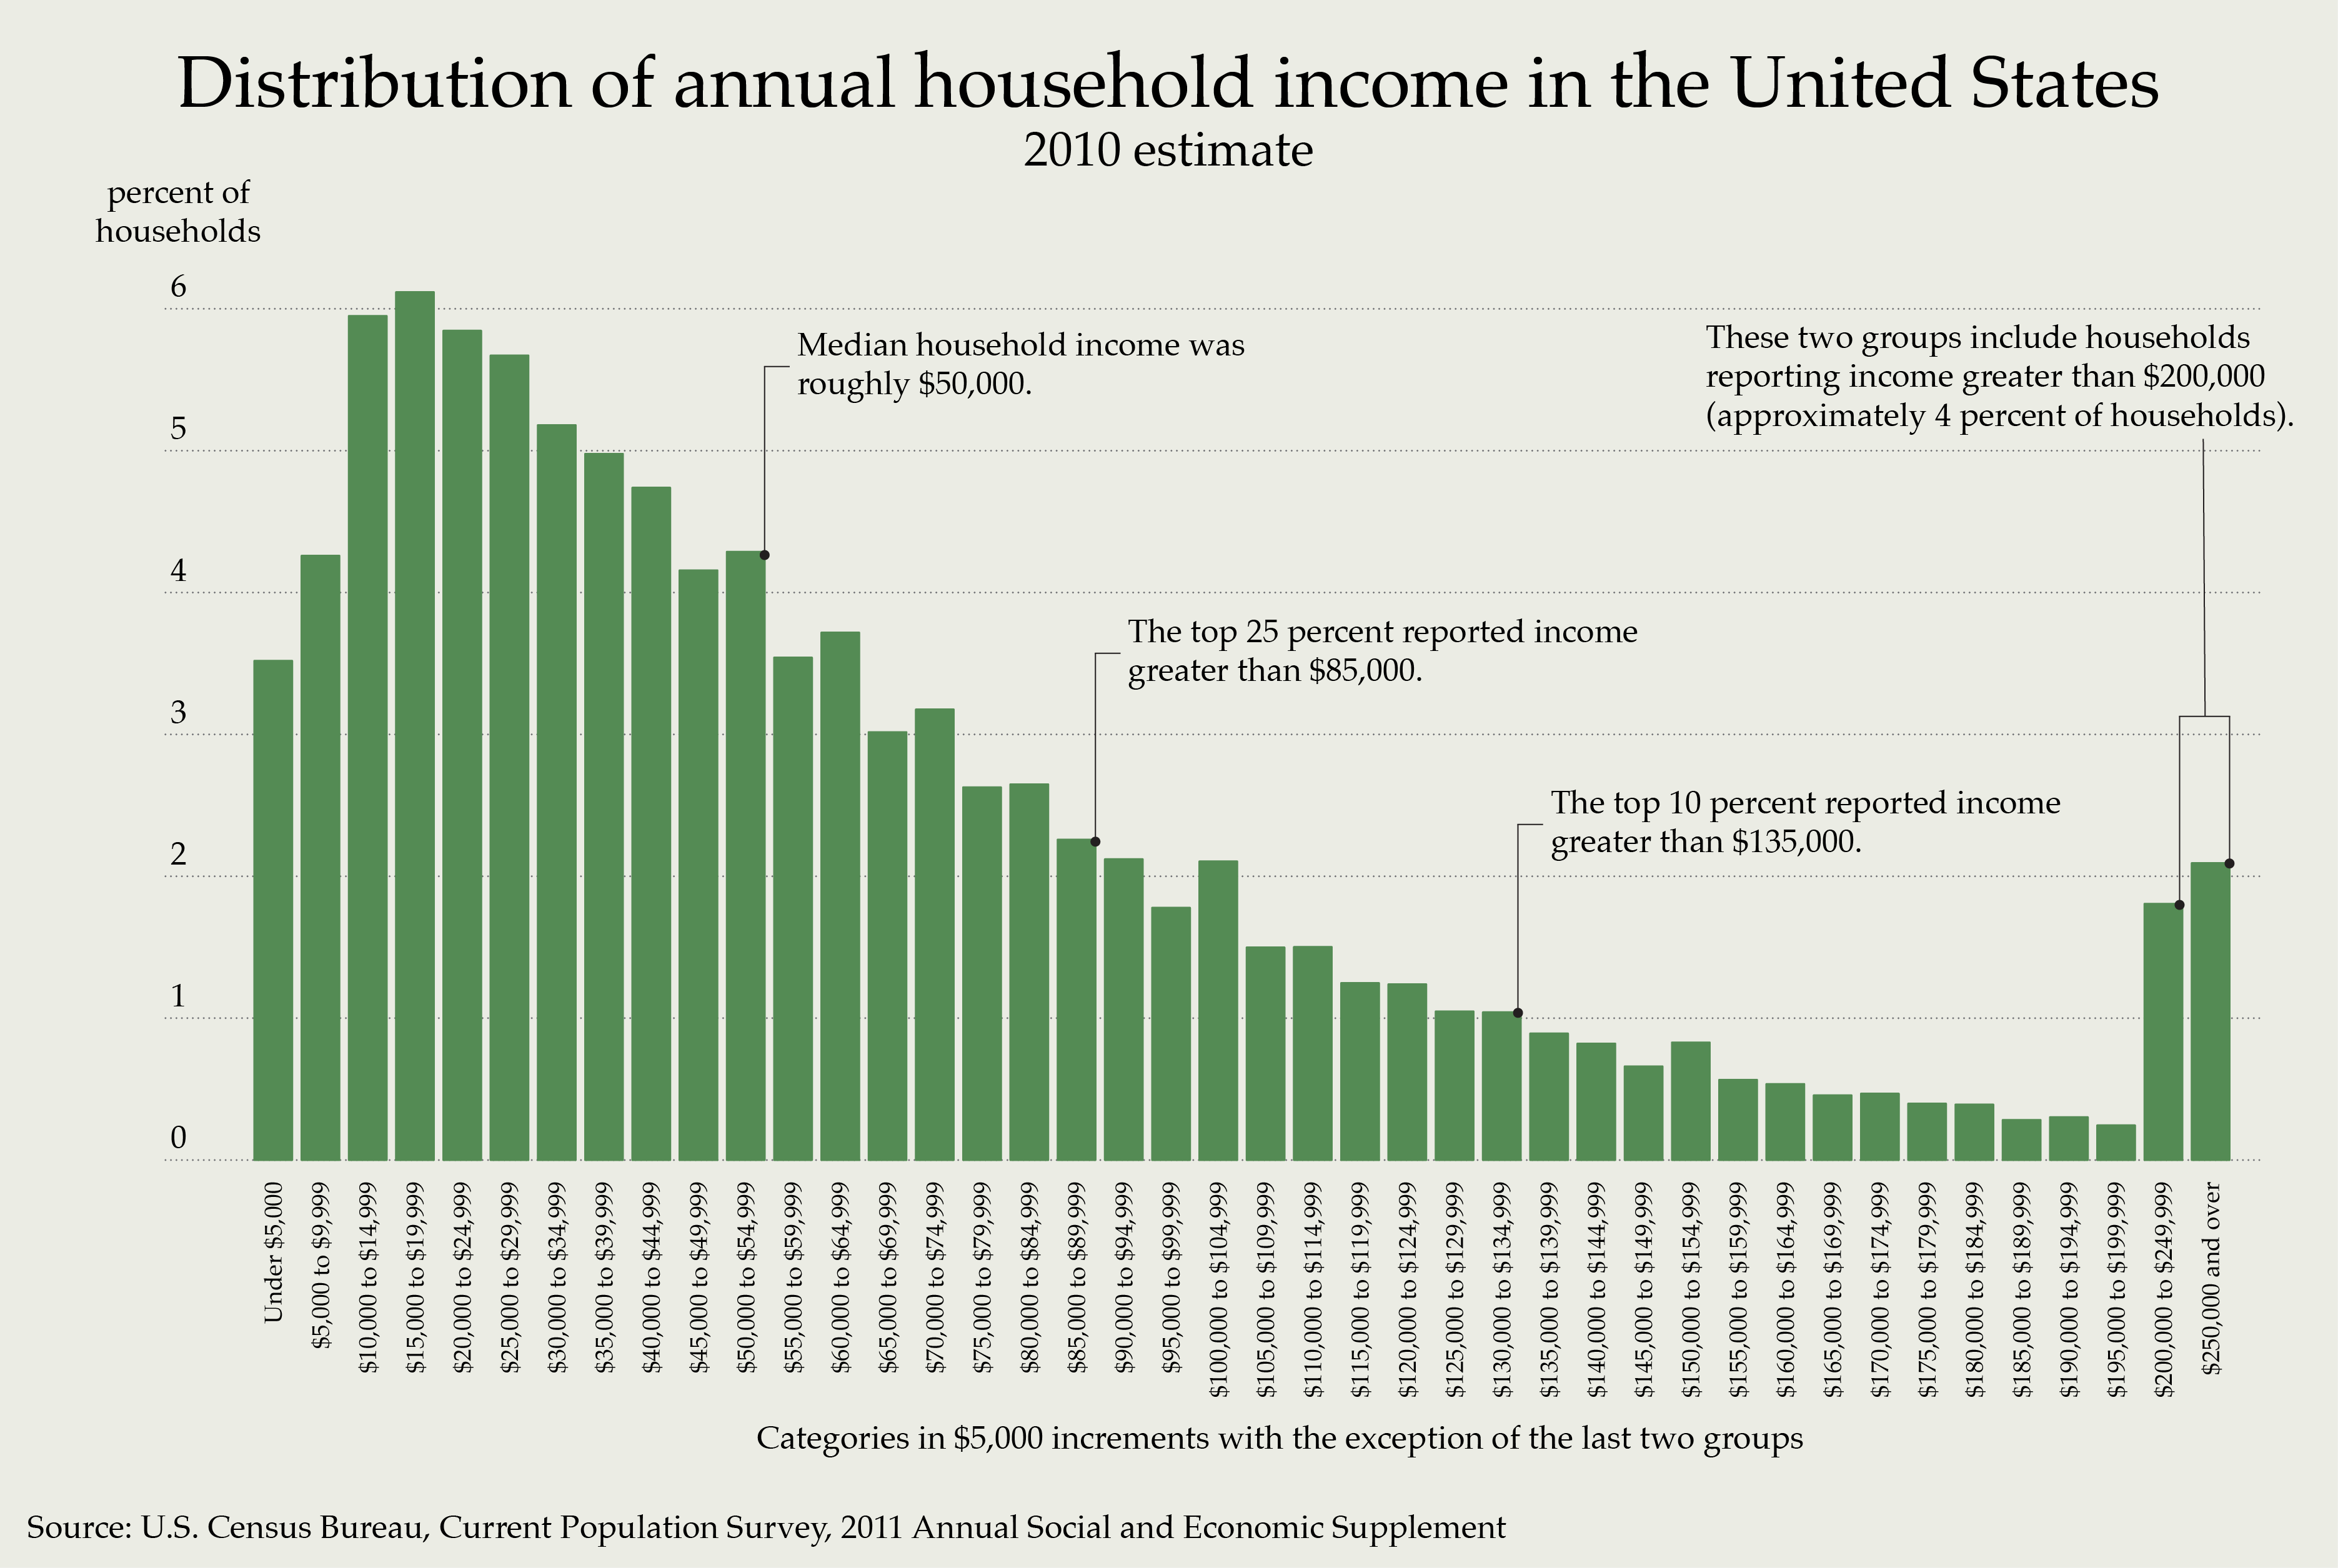
\includegraphics[width=\textwidth]{./figures/Distribution_of_Annual_Household_Income_in_the_United_States_2010.png}
    \caption{Example of a more natural weight distribution with a power law tail but not for smaller weights.}
    \label{fig:natural_weight_distribution}
\end{figure}

% This is particularly true as power laws 
% A sequence of weights with a constant q-tile of largest weights fitting into $\tau$ powerlaw tramlines fits the general GIRG formulation, but could still look quite different based on the distribution of the smaller weights.

An easy improvement for fitting a specific real graph is to take the sequence of node degrees as weights
\footnote{these are now all positive integers $\geq 1$ as opposed to real numbers $\geq x_{\min}$, since in the largest connected componenet, minimum degree is 1}.
This would clearly have better classificaiton performance than power law generating weights.

For the classification comparison framework, Blasius actually uses weight copying for fitting the Chung-Lu GGM, but not for the hyperbolic GGM (which is odd). This doesn't make a fair / like for like comparison, so we cover all bases by having both weight copied and power law fit GIRGs, as well as adding in power law fit Chung-Lu. ER and BA GGMs are of course just fit on the courser metric of overall graph average degree.

Comparing weight copied Chung-Lu with weight copied GIRGs was additionally interesting as their classification from real graphs was harder and hence more informative (trying to compare a 97\% vs 99\% classification accuracy is less meaningful than a 80\% vs 90\%).

% (QUESTION: does the GIRG formulation actually guarantee that as n -> infinity you couldn't tell the difference? I don't think so. E.g. if 1/4 of nodes had w=1, 1/4 had w=10 and 1/2 were power law above 10 distributed.)


\begin{comment}
Integrating $\int_w w^{-\tau} \PP(\Poisson(\Theta(w)) = x) dw$ gives $\E[dd(x)] = \Theta(x^{-\tau})$, for large $x$, dropping smaller order terms.


If instead, independently, each $d_u = \E[\Poisson(\Theta(w_u))] = \Theta(w_u)$, then we would sort of be able to say that the degree distribution follows a $\tau$ exponentiated power law distribution.
We would argue that independently, $P(d_u=m) \approxeq \Theta( \int_{m-1/2}^{m+1/2} w^{-\tau}) = \Theta(m^{-\tau})$, and hence that $dd(m) \sim \frac{Bin(n, m^{-\tau})}{n} \to N(m^{-\tau}, \frac{m^{-\tau}(1- m^{-\tau})}{n}) \approxeq m^{-\tau}$.

Ok so now if $d_u \sim \Poisson(\Theta(w_u))$, can we then derive $\PP(d_u = d)$? $\PP(d_u = d) = \int_W \PP(d_u = d | w_u = w) p(w) dw$. For large $w$, we approximate $\Poisson(\Theta(w_u)) \approxeq N(\Theta(w_u), \Theta(w_u))$. Hence we get $\PP(d_u = d) \propto \int_W \exp(-\frac{(w-d)^2}{2w}) w^{-\tau} dw$. We approximate this integral to be dominated by the interval $w \in [d - k\sqrt{d}, d + k\sqrt{d}]$ for sufficiently large $k$.

So we get $\PP(d_u = d) \propto \int_{d - k\sqrt{d}}^{d + k\sqrt{d}} \exp(-\frac{(w-d)^2}{2w}) w^{-\tau} dw \approxeq \int_{d - k\sqrt{d}}^{d + k\sqrt{d}} \exp(-\frac{(w-d)^2}{2d}) w^{-\tau} dw$. 

Substitute in $x = w - d$ to get $\int_{-k \sqrt{d}}^{k \sqrt{d}} (d + x)^{-\tau} e^{-x^2/2d}dx$.

Then using $(d + x)^{-\tau} = d^{-\tau} (1 + \frac{x}{d})^{-\tau} \approxeq d^{-\tau} (1 - \frac{\tau x}{d} + \frac{\tau(\tau+1)}{2} \frac{x^2}{d^2})$ for $x \in [-k \sqrt{d}, k \sqrt{d}]$, we get $\int_{-k \sqrt{d}}^{k \sqrt{d}} (d + x)^{-\tau} e^{-x^2/2d}dx \approxeq d^{-\tau} \int_{-k \sqrt{d}}^{k \sqrt{d}} (1 - \frac{\tau x}{d} + \frac{\tau(\tau+1)}{2} \frac{x^2}{d^2}) e^{-x^2/2d}dx$.

Finally we can use the results on the pdf of a normal distribution integrating to $1$; the mean integrating to $0$, and the variance integrating to $\sigma^2$, to get that $\PP(d_u = d) \propto d^{-\tau} (1 + \frac{\tau(\tau + 1)}{2} d^{-2} d) = d^{-\tau} 1 + \frac{\tau(\tau + 1)}{2} d^{-(\tau + 1)}$. This formula is essentially a weighted average between two different power law distributions. As $d \to \infty$ it will actually be correct, and be dominated by the larger $d^{-\tau}$ term. However for not so large $d$, it will be more a mix, and so the "perceived/empirical" powerlaw exponent could look larger, presumably somewhere in $[\tau, \tau + 1]$.


None of this is quite true as $d_u$ aren't independent: doubly so, 1. due to weights, and 2. due to positions. 

Hence for a GIRG, $ \E[dd(x)]  \propto x^{-\tau}$ for $x_\text{min} < x \in \N$, a lower cutoff point. This cutoff is necessary not just because the pdf would blow up at $x=0$, but also because the power law behaviour may only hold for higher degrees. The GIRG 
\end{comment}


\subsection{Fitting $c$ and $\alpha$}
These are our last two GIRG parameters to fit.
The parameter $c$ is most directly linked to the generated graph's average degree, whereas the parameter $\alpha$ is more linked to the power of the geometry - larger $\alpha$ decreases the probability of longer distance edges which have $\rho_{uv} < 1$, leaving edges more dominated by shorter (and more geometric, clustered) edges. We hence follow \cite{blasius2018towards} by fitting $\alpha$ with the clustering coefficient. Unfortunately in our experiments we used the (average) local clustering coefficient (LCC) to fit our GIRGs and Hyperbolic Random Graphs, 

\begin{equation}
    \mathrm{LCC}(G) := \frac{1}{|V|} \sum_{u \in V} 
    \frac{| \{ v, v' \in \Gamma(u): v \sim v'\} |}{{|\Gamma(u)| \choose 2}}
\end{equation}
instead of the global clustering coefficient as in \cite{blasius2018towards}. The global clustering coefficient, the fraction of total "V" shapes that indeed are completed as full triangles is likely a better metric than the LCC. Luckily in practice they generally differ by less than $1\%$.

Unfortunately $c, \alpha$ are not wholly independent, so we must fit them in tandem, fitting $c$ for a given $\alpha$ so as to match the average degree of $G$, and then $\alpha$ for that given $c$ to match the LCC of $G$. This then looks like coordinate ascent in 2D, we alternatively maximise $c \gets \hat{c}_1;\; \alpha \gets \hat{\alpha}_1;\; c \gets \hat{c}_2;\; \alpha \gets \hat{\alpha}_2;\; ...$.

Fitting $\alpha \gets \hat{\alpha}_i$ based on LCC is precisely ABC like - we propose potential $\alpha_i$ values using binary search, for which we generate a graph $G' \sim \cG_{\GIRG}(n, d, \hat{c}_i, \alpha_i, \tau)$, and use the distance $|\mathrm{LCC}(G') - \mathrm{LCC}(G)|^2$. To both propose the next candidate $\alpha_i$ and eventually accept the final best $\hat{\alpha}_i$.

\cite{blasius2022efficiently} luckily gives a more efficient method to fit $c$ given $\alpha, d$, and a pre-sampled set of weights $(w_u)_{u \in V}$, that doesn't involve fully sampling a new $G' \sim \cG_{\GIRG}$. They derive a formula for the expected average degree $\E[\overline{deg}]$ of the GIRG.
\begin{equation}
    \label{eq:expected_edge_degree}
    f(c) = c A + c^{1/\alpha} B
\end{equation}
Hence we just have to numerically solve \cref{eq:expected_edge_degree} for $\hat{c}: f(\hat{c}) = \overline{deg}$ in order to obtain our desired average degree $\overline{deg} = 2|E|/|V|$.

The expected average degree formula of \cref{eq:expected_edge_degree} miraculously holds for all volume based toroidal GIRGs (regardless of exact disance function $r(x_u, x_v) = r_{uv}$), and we can even adapt the formula to be independent of dimension $d$.

\paragraph{Derivation of GIRG expected average degree formula}
The volume formulation of a GIRG presents a useful generalisation:
\begin{equation}
    p_{uv}(r) = \min \left \{ 
        1,
        c \left (
            \frac{w_u w_v / W}{Vol(r_{uv})}
        \right )^\alpha    
    \right \}; \quad \rho_{uv} = \frac{w_u w_v / W}{Vol(r_{uv})}
\end{equation}
Here $Vol(r_{uv}) = Vol(B_{r_{uv}})$ is the volume of the ball of radius $r$ using the distance function $r(x_u, x_v) = r_{uv}$, which must be symmetric to make sense.
For example in the $\infty$-norm, $Vol(r_{uv}) = (2r_{uv})^d$ as a cube with side-length $2r_{uv}$.

Having volume in the edge probability formula is actually a generalisation of taking $r_{uv}$ to the dth power - the point being to make $p(u \sim v | x_u, w_u, w_v) = E_r[p_{uv}(r)] = \Theta(w_u w_v/n)$, regardless of dimension.
So we'll derive $E_r[p_{uv}(r)]$ for a general volume function $Vol(r)$, and fixed weight sequence $(w_u)_{u \in V}$ and use this to recover \cref{eq:expected_edge_degree} via $E[\overline{deg}] = \sum_{u \in V} \frac{1}{n} \sum_{v \in V} E_r[p_{uv}(r)]$.

% We'll derive the same resultant $p(u \sim v | w_u, w_v) = \E_r[p_{uv}(r)]$ regardless, relying only on the fact that $Vol(r)$ is an increasing function. Finally, $\E[d_u] = \sum_v p(u \sim v | w_u, w_v)$ and hence $\E[\overline{deg}] = \sum_u \E[d_u]$.

Now $E_r[p_{uv}(r)] = \int_r p_{uv}(r) p(r) dr$. We'll break this down into $\int_{r: \rho_{uv} \geq 1} + \int_{r: \rho_{uv} < 1}$, and write $\hat{r} : Vol(\hat{r}) = \frac{w_u w_v}{W} c^{1/\alpha}$ as the boundary radius at which $\rho_{uv} = 1$.

Hence we get $E_r[p_{uv}(r)] = \int_0^{\hat{r}} p(r) dr + \int_{\hat{r}}^{r_{\max}} p_{uv}(r) p(r) dr$.

Substituting $Vol = Vol(r);\; dr = dVol \frac{dr}{dVol} = \frac{dVol}{p(r)}$, we get:

\begin{align}
    E_r[p_{uv}(r)] =& 
    \int_0^{Vol(\hat{r})} dVol + 
    \int_{Vol(\hat{r})}^{Vol(\mathbb{T})} p_{uv}(Vol) dVol
    \\
    =&
    Vol(\hat{r}) + 
    \int_{Vol(\hat{r})}^{Vol(\mathbb{T})} 
    c \left (\frac{w_u w_v}{W} \right )^\alpha Vol^{-\alpha}  
        dVol
    \\
    =&
    Vol(\hat{r}) + 
    c \left (\frac{w_u w_v}{W} \right )^\alpha \frac{1}{\alpha - 1}
        \left [
            \left (\frac{w_u w_v}{W} \right )^{1 - \alpha} c^{\frac{1 - \alpha}{\alpha}} - 1
        \right ]
    \\
    =&
    c^{1/\alpha} \left (\frac{w_u w_v}{W} \right ) 
        \left [ 1 + \frac{1}{\alpha - 1} \right ] 
    - 
    \frac{c}{\alpha - 1} \left (\frac{w_u w_v}{W} \right )^\alpha
    \label{eq:p_u_to_v_marginal_on_position}
\end{align}
Where in the last two lines we sub in $Vol(\hat{r}) = c^{1/\alpha} \left (\frac{w_u w_v}{n} \right )$, and $Vol(\mathbb{T}) = 1$.
I.e. across all GIRGs of different distance functions and dimensions $d$, we get the same resultant edge probabilities when marginalising out node locations - and $\Theta(\frac{w_u w_v}{W})$ as promised!

Following \cite{blasius2022efficiently} Appendix, the formula just needs a correction for pairs $u, v$ such that $Vol(\hat{r}) = c^{1/\alpha} \left ( \frac{w_u w_v}{n} \right ) > 1$, wherein the second integral is unnecessary, and the first is capped lower at $1$, the volume of the Torus. These are pairs $u, v$ which have such giant weights $w_u, w_v$ that $p_{uv}(r) = 1$ identically, no matter how far apart $x_u, x_v$ are placed in the Torus.

% Finally the average degree formula in \cref{eq:expected_edge_degree} is just averaging over all terms in \cref{eq:p_u_to_v_marginal_on_position} for each pair of vertices $u, v$.


% The more general formula replaces replaces $||x_u - x_v||^d = r_{uv}^d$ with $Vol(B_r)$ the volume of the ball of radius $r=r_{uv}$.
% For norms, $Vol(B_r) = \Theta(r^d)$, e.g. in the $\infty$-norm, $Vol(B_r) = (2r)^d$ as a cube with side-length $2r$.
% The euclidean ball has some $\pi$'s in the formula. For the minimum component distance, $Vol(B_r) = \Theta(r)$.
% Volumetric equivalence makes sense in that the edge probability $p_{uv} | x_u, w_u, w_v$ in the Torus is determined by integrating $\int_{r=0}^{r=1} p_{uv}(r) p(r) dr = \int_{Vol=0}^{Vol=1} p_{uv}(Vol) dVol$, where $Vol(r) = Vol(B_r)$ is the volume of the ball of radius $r$.
% Hence across different GIRGs of different dimensions $d$, keeping $p_{uv}(Vol)$ the same function therefore keeps the pairwise edge probabilities $p_{uv}$ the same (but not the joint edge probability distribution of course).




\section{Cube GIRGs}

Cube GIRGs are an alternative formulation to Toroidal GIRGs. Instead of the $d$-dimensional torus $\chi = \mathbb{T}^d$, we have the $d$-dimensional cube $\chi = [0,1]^d$. Thus the tradeoff is to lose the symmetry and simplicity of the torus, for the ability to hopefully generate more realistic graphs, as few situations in the real world are Toroidal.

% For example with our socfb social network graphs, likely geometric quantities are home address (as a 2d vector location - these networks are from a small town/city/university - only on planet earth scale do geographic locations become somewhat more toroidal), political leaning (typically a 2d axis of economic left/right, and authoritarian/libertarian - e.g. an extreme authoritarian is unlikely to get along with an extreme libertarian), athletic proclivity etc. all generally are non toroidal. Perhaps one toroidal-esque quantity could be that in all cases, a pair of positive and negataive far out leaning people share in common their marginalisation / non conventionality - this could potentialily be captured on a 1D non toroidal normie vs hipster scale.  

For example with our socfb social network graphs, likely geometric features for each individual are home address, age, athletic proclivity, political leaning etc.
In the environ of a town/city, home address is a 2D vector (only whole planet scale geographic locations look more torus-esque).
Age and athleticisim are clearly both non toroidal (and hence cube like) quantities.
Political leaning could be e.g. a 2d axis of economic left/right and authoritarian/libertarian. This might bear a toroidal-esque quantity two individuals on far opposite extremes of an axis share some common ground, e.g. a hardcore communist and a fascist might both share values such as railing against the status quo, or enjoying political rallies. No model is perfect; this could potentially be captured as an extra (non toroidal) feature dimension placing individuals on a scale of normie to hipster.

\subsection{Cube GIRG Formulation}
The neat correspondence between volume and distance unfortunately breaks down when translating from torus GIRGs to cube GIRGs, due to the loss of spatial symmetry. Where before we could write e.g. $Vol(r_{uv}) = (2 \norm{x_u - x_v})_\infty^d$, now in cube geometry $Vol(B_{r_{uv}}(u)) = Vol(B_{r_{uv}}(u)) \cap [0, 1]^d$, i.e. volume only counts within the cube itself, and hence oftentimes $Vol(B_{r_{uv}}(u)) \neq Vol(B_{r_{uv}}(v))$. 

We will use a simpler cube GIRG formulation based solely on distance, i.e. the factor of $r_{uv}^d$ in $p_{uv}$. This is conceptually easy to understand, and allows for a neat coupling with the original Torus geometry whereby $r_{uv}^C \geq r_{uv}^\T$, with most pairs having $r_{uv}^C = r_{uv}^\T$. We can say that a GIRG in cube geometry is stochastically dominated by its torus geometry counterpart (and hence strictly sparser). 

A volume based formulation of edge probabilities is more complicated - it could look something like replacing $Vol(r_{uv}) \mapsto \sqrt{Vol(B_{r_{uv}}(u)) Vol(B_{r_{uv}}(v))}$.
Intuitively in the social network analogy, this is like saying that all people, no matter how extreme their geometric location, have the same desire to make friends (modulo their inhomogeneous weights as that is the literal introversion / extroversion factor in the GIRG model).
Thus if we were modelling directed edges, we could have equality in $E_r[p_{u \to v}(r)]$ in all GIRGs of differing distance metric, number of dimensions and torus / cube geometry by using volume based formulations.
Unfortunately desire to make friends doesn't equate to actual friends, as they have to want you back.
So if a node $u$ is near the edge of the cube, it may send out the normal volume based amount of friendship invitations ($u \to v$), but if most of these go to nodes $v$ nearer the centre of the cube, fewer will reciprocate ($v \to u$). In the torus geometry (all weights being equal), every $u$ would have the same expected number of outgoing edges as incoming. The volume based cube GIRG formulation would still have higher average degree than the distance based version, but lower than the torus.

% however if an undirected edge $u \sim v$ requires both $u \to v$ and $u \gets v$, so even if $u$ has many outgoing friendship invitations, if all its proposed friends have many friendship options ($u$ is the mountain cave hermit soliciting friends in the nearby village), $u$ will still end up with fewer friends than average, however more than in the distance based formulation:

% We will use a simpler cube GIRG formulation based solely on distance, i.e. the factor of $r_{uv}^d$ in $p_{uv}$. This is conceptually easy to understand, and allows for a neat coupling with the original Torus geometry whereby $r_{uv}^C \geq r_{uv}^\T$, with most pairs having $r_{uv}^C = r_{uv}^\T$. We can say that a GIRG in cube geometry is stochastically dominated by its torus geometry counterpart (and hence strictly sparser). 


% $r_{uv}^C$ vs $r_{uv}^\T$ in a cube vs torus satisfies $r_{uv}^C \geq r_{uv}^\T$. For the $\infty$ norm, $r_{uv}^C = r_{uv}^\T \iff r_{uv}^C \leq \frac{1}{2}$. The simplest edge probability translation therefore is just to use the same $r_{uv}^{-d \alpha}$ factor, such that Cube GIRGs are just a more sparse version of Toroidal GIRGs. We call this the distance based formulation. 

% An alternative volume based formulation, seeking to replicate the $r_{uv}^d \propto Vol(B_{r_{uv}})$, is complicated by the lack of symmetry. The whole point of the general volume formulation of edge probability was that the node $u$ has a set edge probability to neighbours $v$ at a certain volumetric distance - where now in the cube case, we could take $Vol(B_{r_{uv}}(u)) = Vol(B_{r_{uv}}(u)) \cap [0, 1]^d$, i.e. volume only counts within the cube itself.
% This is not symmetric in that $Vol(B_{r_{uv}}(u)) \neq Vol(B_{r_{uv}}(v))$: if $u$ is closer to the edge of the cube and $v$ closer to the centre, then $Vol_u < Vol_v$.
% However dealing with undirected edges, we must have one agreed upon formula for $p_{uv}(r)$, and so a natural formula would be to replace $Vol(B_{r_{uv}}) \mapsto \sqrt{Vol(B_{r_{uv}}(u)) Vol(V_{r_{uv}}(v))}$. This would basically seek to compensate a $u$ near the edge, allowing it to better seek far away neighbours.
% Even still, this does not end up with all nodes of a weight having the same expected number of neighbours regardless of their location. Rather it's like we had directed eges, yielding undirected edges if both directions are present: $u \to v$ and $v \to u$ implies $u \sim v$. With this volume based formulation, every node has out edges based on its own weight and volumetric distance to other nodes. $p(u \sim v) = p(u \to v) p(v \to u)$. If we ignored the minimum term in the edge probabilities (i.e. saying that $p(u \to v) \propto w_u / \sqrt{Vol(B_{r_{uv}}(u))}$, not upper bounded by $1$, then actually all nodes would have the same expected number of neighbours, regardless of their location.

% In the social network analogy, the distance based formulation is like saying that people make friends only with those who live close by.
% Thus if a person lives like a hermit in a mountain cave far from the neaerest village, they're unlikely to have many friends.
% The volume based formulation is saying that all people, no matter how extreme their geometric location, have the same desire to make friends (holding their inhomogeneous weights constant, as that is the literal introversion / extroversion factor in the GIRG model). So even if you're the most far left communist, you will still make as much total social effort, primarily on far lefters, but also towards even some centre left potential friends. However to most central leftists, the communist is too extreme and won't get much social budget compared to the large choice of more politically nearby folks.

% TODO think more if good idea?
% Another possible model for spheres of influence about nodes near the edge of the cube is one where spheres of influence are no longer radially symmetric. In the volume based formulation in a 2D space, where $u$ is near the north edge of the square, efforts to find friends in the north are redirected equally along the east, south and west at the same radius. In a physical analogy, it's possible instead that "feelers" to the north are redirected along the path of least resistance, to the east and west. In a political spectrum analogy, more aligned to the min GIRG philosophy, if a person is located in the far social left of the cube, but economically central, they may seek friendships amongst those who are either similarly economically or similarly socially. Hence if there are no people more socially left, they may redirect their social dimension friendship effort budget to those a bit more socially right of themselves, rather than also to those economically left/right close by. We don't pursue this model!

\subsection{Cube GIRG generation - coupling algorithm}
We use the distance based cube GIRG formulation, which permits a simple coupling based generation algorithm off of an already generated Torus GIRG, shown in \cref{alg:cube_coupling}. This runs in $O(n)$ extra time on top of the initial Torus GIRG generation.

\begin{algorithm}
    \caption{Generate Cube GIRG from Torus via coupling}\label{alg:cube_coupling}
    \begin{algorithmic}
    \Require $n$, $d$, $c$, $\tau$, $\alpha$
    \State $\left ( G, \{x_u\}_{u \in V}, \{w_u\}_{u \in V} \right ) \gets \text{torus-}\GIRG(n,d,c,\tau, \alpha)$
    \For{$(u,v) \in E(G)$}
        \State $p_{uv}^\T = \min \{1, c \left (
            \frac{w_u w_v / W}{(r_{uv}^\T)^d} \right )^\alpha \}$
        \State $p_{uv}^C = \min \{1, c \left (
            \frac{w_u w_v / W}{(r_{uv}^C)^d} \right )^\alpha \}$
        % \If{$p_{uv}^C < p_{uv}^\T$}
        % \State $p_{\text{del}} \gets 1 - \frac{p_{uv}^C}{p_{uv}^\T}$
        \State $p \gets U[0,1]$
        \If{$p > \frac{p_{uv}^C}{p_{uv}^\T}$}
            \State delete edge $(u,v)$ from $G$
        \EndIf
        % \EndIf
    \EndFor
    \State \Return $G$
\end{algorithmic}
\end{algorithm}



\subsection{Estimating const $c$ in Cube GIRGs}
To fit $c$ for a specific real graph $G$, for Torus GIRGs we solved for the equation $f(c) = \overline{deg}$, given fixed $\alpha$. Our distance based Cube GIRGs have fewer edges in expectation than their toroidal counterparts, and no nice formula for the expected average degree. Instead we estimate $\hat{c}$ by starting with an initial guess $c_0: f(c_0) = \overline{deg}$, and iteratively updating by each time generating a graph $G_i \sim \GIRG(c_i)$ and setting $c_{i+1} \gets c_i \frac{n \overline{deg}}{2 |E(G_i)|}$ until convergence.


\section{Min GIRGs}
In \cref{sec:GIRG_def} we introduced the max norm $\norm{\cdot}_\infty$, euclidean norm, and the minimum component distance (mcd) $\norm{\cdot}_{\mathrm{mcd}}$ as alternative distance functions.
While the max norm is commonly used in e.g. \cite{bringmann2019geometric} as its handy for proofs, the mcd can make more sense in some settings. For instance in social networks, the max norm is like stipulating that people only make friends with others that "tick all the boxes", i.e. are similar in every dimension (this sounds more like finding a romantic partner). The mcd is saying that you make friends with people who are similar in at least one dimension. E.g. an individual might play in the local football club, and sing in the local choir - each a social circle formed from one shared hobby.

The mcd can be mixed with the max norm in an "and/or" fashion, e.g. $\norm{x - y} = \norm{z} = \min \left ( z_1, \max (z_2, z_3), \max (z_4, z_5) \right )$.
This parses as points $x, y$ being "close" if they are close in the 1st dim, or the 2nd and 3rd dim, or the 4th and 5th dim.

\section{Blasius classification results}
% TODO
% \begin{enumerate}
%     \item table of classification accuracies vs real-world
%     \item explanation of copyweight GIRGs, normal GIRGs, cube GIRGs, min GIRGs, mixed GIRGs
%     \item analysis of which features different models seem to be good at
%     \item table of classification accuracies vs 1D GIRGs
%     \item analysis of which features different dimensional GIRGs seem to be distinguishable on
%     \item 
% \end{enumerate}

As introduced in \cref{sec:ggm_blasius_framework}, we fit a selection of GGMs, including various different kinds of GIRG on around 100 socfb Facebook graphs, whose sizes range from $1000$ to $100,000$ nodes. For each GGM we produce a mirrored dataset of fake graphs, with which we train a sequence of SVM classifiers to distinguish between the real and fake datasets, differing on which high level graph features they use as input. Higher classification accuracies, e.g. $99\%$, denote that the GGM generates are readily distinguishable from the real graphs, and hence the GGM is a poor / unrealistic fit; $50\%$ accuracy is the gold standard of real/fake indistinguishability on the feature set.

We can see from \cref{fig:blasius_framework_table} that mimicking the features of real Facebook graphs with generations from a fit GGM is tough. For example in the feature set (n, m, deg), by deg we mean to include 5 numbers per graph: mean node degree; lower, middle (median) and upper quartile node degree, and standard deviation over all node degrees. Our numbers can be compared to Table 2 in \cite{blasius2018towards}, which also includes feature sets with just mean node values, which in some cases makes fooling the classifier much easier\footnote{We do get similar results to Table 2 when training SVMs with just the mean node features, which can yield lower accuracies in the $50-70\%$ range}.

Features like k-cores and comms aren't node level, and are taken over the actual core/community sizes - so are e.g. mean, median etc. community sizes within a graph.

% seem low in places compared to \cite{blasius2018towards}, which is because we have a higher bar due to a more extensive feature set. For exmaple in the feature set (n, m, deg), by deg we include 5 numbers per graph: mean node degree; lower, middle (median) and upper quartile node degree, and standard deviation over all node degrees; \cite{blasius2018towards}'s Table 2 uses just mean value for node level features \footnote{We do get similar results to Table 2 when training SVMs with just the mean node features, which can yield lower accuracies in the $50-70\%$ range}. Features like k-cores and comms aren't node level, and are taken over the actual core/community sizes - so are e.g. mean, median etc. community sizes within a graph.

\paragraph{Types of GIRG tested in classification framework} The base GIRG type we tried was max norm torus GIRGs for dimension $d$ from $1$ to $7$. Note only $d=1, 2, 7$ are shown in \cref{fig:blasius_framework_table} as the classification numbers follow a trend in dimension.

We also tried mcd torus GIRGs for $d=2,3,4,5$ ($d=1$ is equivalent to max norm), as well as min/max mixed torus GIRGs with mixing $1-23$, $1-234$, $12-34$, $1-2-34$. The latter two are excluded from \cref{fig:blasius_framework_table} as they had worse classification numbers.

Finally we trained some max norm cube GIRGs - though we were held back due to the increased computation when fitting the average degree with constant $c$. Hence we just had $d=1,2,3$ cube GIRGs, and $d=1,2,3,4,5$ copy-weight cube GIRGs (an attempt for maximal realism).

Finally we have the host of simpler models CL, BA, ER as in \cite{blasius2018towards}, as well as Hyperbolic Random Graphs which are very similar to 1d-GIRGs.


\paragraph{(effective) diameter}
Only the features diam and eff-diam  are single numbers per graph - as just one number this is easier to mimick, e.g. the 2d, 3d cube GIRGs get $77\%$ accuracy. cube GIRGs' having a more realistic effective diameter than torus GIRGs could just be a result of torus GIRGs having too small diameters compared to real graphs, and cube GIRGs having larger diameter than toroidal\footnote{Looking at the features of real and generated graphs, the effective diameter of the FB graphs range from $3.0$ to $4.4$; 2d torus GIRGs on average $0.17$ less than their real counterparts, and 2d cube GIRGs just $0.04$ less.}. This does however fit our geometric intuition of the realism of cube geometry over toroidal.

\paragraph{closeness centrality}
To draw another example, for the n, m, close feature set, 2d GIRGs only achieve 98\% accuracy. This is just slightly better than CL, BA, ER, but still seems very bad. However \cref{fig:real_2d_closeness_mean_scatter} shows that mean closeness fits very accurately to the real graphs. Nonetheless, due to a consistently lower standard deviation of closeness in the GIRGs and the fact that the standard deviation of closeness in real graphs fits well as a function of number of nodes, the 2d GIRGs are distinguishable from real graphs on this feature set. I would argue that 2d GIRGs did a pretty good job on replicating closeness in real graphs, so the high accuracy of 98\% is a little misleading.

Classification accuracy is a crude metric, but should at least be a point of comparison between GGMs. 
A drawback of this framework is that the attainable accuracy is also affected by the variety / predictability of a feature set across the real graph dataset - whatever the real graphs are doing, the GGMs have to do too - but more variance is easier to blend in with than a strict pattern. Our GGMs furthermore are much more likely to produce a set of similar graphs following a strict pattern.

\paragraph{GIRGs performance}
We can compare classification performance between different types of GIRGs, as well as between GIRGs and other GGMs; Chung-Lu acts as a good null hypothesis for GIRGs without geometry\footnote{Another potential GGM geometry null hypothesis would have been the configuration model which tries to mimick a degree sequence, like Chung-Lu, but more strictly. Each node is given a set number of "half edges" which gives it a set degree (the degree sequence can be random e.g. power law generated, or given e.g. copied directly from a real graph. Half edges are then joined together at random.)}.

Copy-weight cube GIRGs have a clear cut performance advantage over all other GGMs, only rivalled by copy-weight Chung-Lu. We see, as expected, improvements in diameter and effective diameter over Chung-Lu, and just in effective diameter for non copy-weight GIRGs. Copy-weight GIRGs also have improved LCC performance over copy-weight Chung-Lu, though this is not observed in powerlaw weighted GIRGs - despite explicitly fitting the mean LCC, the wider LCC statistics must be quite distinguishable. 

Not-surprisingly copy-weight GGMs have very good degree distribution performance, with Chung-Lu being the best as having no extra geometric modification on the copied degree sequence.

Community sizes and k-core sizes are potentially less consistent features to consider as they have higher variance than node level features.


% The first column of copy-weight cube GIRGs in \cref{fig:blasius_framework_table} have much better classification accuracy than the rest, apart from copy-weight Chung-Lu, which serves as the non-geometric comparison point. It would also be interesting to these GIRGs with the configuration model \footnote{Each node is given a set number of "half edges" which gives it a set degree (the degree sequence can be random e.g. power law generated, or given e.g. copied directly from a real graph. Half edges are then joined together at random.)} with copied degrees as the "null hypothesis" against these.

% In notably geometric feature categories like LCC, and diameter GIRGs indeed out perform Chung-Lu.
% Chung-Lu does better on community size statistics; communities could arguably spring from geometry, but GIRGs' uniformly random geometry isn't really designed for this - you could rather imagine a more realistic setup if node locations were taken from a mixture of gaussian distributions (e.g. a university town might have age/occupation clusters of student age vs working age, or academic vs non-academic peoples).






\begin{figure}
    \centering
    \begin{subfigure}{0.49\textwidth}
    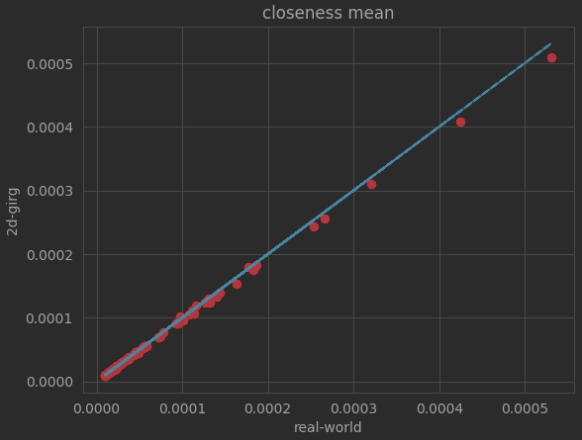
\includegraphics[width=\linewidth]{./figures/real_2d_closeness_mean_scatter.png}
    \caption{2d GIRGs have almost identical mean node closeness to real-world FB graphs; $y=x$ line shown in blue.}
    \label{fig:real_2d_closeness_mean_scatter}
    \end{subfigure}
    \begin{subfigure}{0.49\textwidth}
    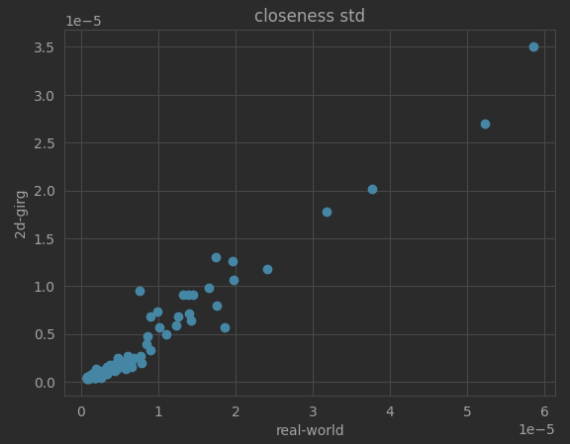
\includegraphics[width= \linewidth]{./figures/real_2d_closeness_std_scatter.png}
    \caption{2d GIRGs have consistently lower standard deviation of node closeness than real-world FB graphs}
    \end{subfigure}
    \begin{subfigure}{0.49\textwidth}
    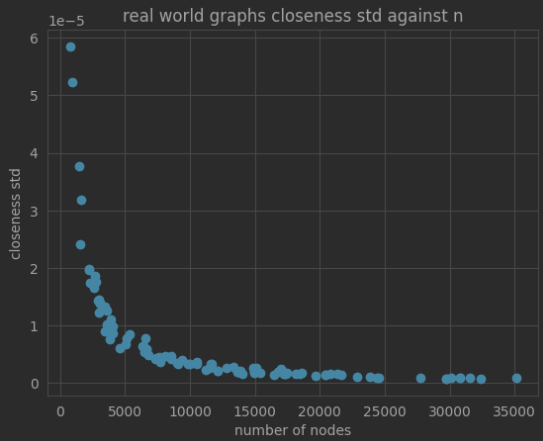
\includegraphics[width=\linewidth]{./figures/real_closeness_std_against_n.png}
    \caption{standrd deviation of node closeness in real-world FB graphs fits well as a function of number of nodes}
    \end{subfigure}
\end{figure}

% (cube GIRGs having slightly larger diameters - to get from one edge of the cube to the opposite), but does fit our geometric intuition.


% does slightly fit our intuition of their more realistic geometry. Funnily enough Cube GIRGs fit on the dataset have 

% just mean that toroidal GIRGs have too large diameters compared to real graph (cube GIRGs having smaller diameters), but does fit our geometric intuition.

% 2+d min girgs we expect to have very large diameters.



\begin{sidewaysfigure}
    \centering
    % \begin{subfigure}
    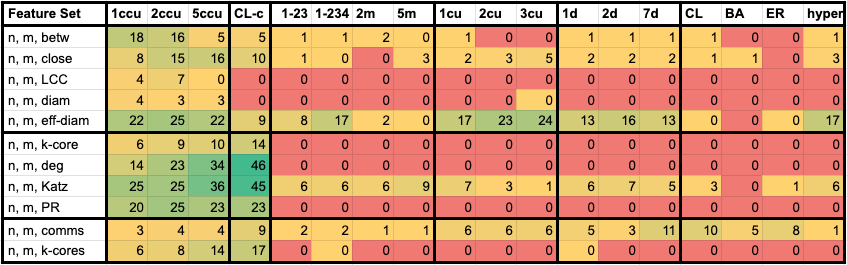
\includegraphics[width=\textwidth]{./figures/Blasius_framework_table.png}
    \caption{\cite{blasius2018towards} GGM comparison framework on Facebook graphs, extended to different GIRG models.
    % If just one of mean/median is used, accuracies are often lower, sometimes even in $50\%-70\%$. $50\%$ is the best possible validation of a GGM as indistinguishable from real data, and is only achieved for feature set $n, m, LCC \;\text{mean}$ (by GIRGs and not the other none geometric GGMs).
    Some models are missing from the table e.g. 3d-6d GIRGs as their results follow a trend from low to high dimension.
    }
    \label{fig:blasius_framework_table}
    % \end{subfigure}
    \vspace{1em}
    \centering
    % \begin{subfigure}
    \begin{tabular}{|c|c||c|c|}
        \hline
        1-ccu & 1d copy-weight cube GIRG 
        & betw & betweenness centrality
        \\
        1-23 & $1 \lor (2 \land 3)$ mixed min/max GIRG
        & k-core & node k-core number
        \\
        2-min & $1 \lor 2$ 2d min GIRG
        & close & closeness centrality
        \\
        3-cu & 3d cube GIRG
        & LCC & node local clustering coefficient
        \\
        7d & 7d GIRG
        & deg & node degree
        \\
        CL & Chung-Lu
        & Katz & node Katz centrality
        \\
        CL-c & copy-weight Chung-Lu
        & PR & node PageRank
        \\
        BA & Barabasi-Albert
        & comms & community sizes
        \\
        ER & Erdos-Renyi
        & k-cores & k-core sizes
        \\
        hyper & Hyperbolic Random Graph &
        diam & graph diameter
        \\
        && eff-diam & graph effective diameter\\
        \hline
    \end{tabular}
    \caption{Graph Generative Model abbreviations; feature name abbreviations}
% \end{subfigure}
\end{sidewaysfigure}

% \begin{sidewaystable}
%     \centering
%     \begin{tabular}{|c|c|}
%         \hline
%         1-co & 1d copy-weight GIRG \\
%         1-23 & $1 \lor (2 \land 3)$ mixed min/max GIRG \\
%         2-min & $1 \lor 2$ 2d min GIRG \\
%     \end{tabular}
% \end{sidewaystable}


% Translating the two equivalent volumetric and distance based formulations of the Toroidal GIRG to the Cube actually gives two different but both potentially sensible definitions. 

% We'll start with the Toroidal Max GIRG where the distance function is $r^\T(x_u, x_v) = \norm{x_u - x_v}_{\infty, \T}$, the derived volume function in the toroidal setting is $Vol^\T(r^\T_{uv}) = (2r^\T_{uv})^d$, and the toroidal edge probability is $p_{uv}(r^\T) = \min \left \{1, \left ( \frac{w_u w_v}{n Vol^\T(r_{uv})} \right )^\alpha \right \} = \min \left \{1, \left ( \frac{w_u w_v}{n (2r^\T_{uv})^d} \right )^\alpha \right \}$. 

% The distance based cube GIRG connection probabilities just replaces $r^\T_{uv}$ with the cube distance $r_{uv}$, which is in general equal, or longer depending on the positions $x_u, x_v$.

% The translation of $Vol^\T(r^\T_{uv})$ into a cube geometry now no longer makes sense without a reference point about which the ball volume is measured. Hence it is replaced with $\sqrt{V_u(r_{uv}) V_v(r_{uv})}$, where $V_u(r_{uv})$ is the volume of the $r_{uv}$ ball about point $x_u$, only including intersection with the cube. This definition partially assuages the reduced connectivity of points $u$ that are near the extremes of the cube - their $V_u(r_{uv})$ is smaller than if they were more centrally located, and hence they strive more strongly to connect - however their potential neighbours $v$ will still usually be more centrally located and hence less willing to reciprocate the connection.

% The upshot connectivity comparison between the Torus and Cube GIRG, is that connection probabilities for centrally located nodes are generally the same. For distance based Cube GIRGs, connection probabilities everywhere are upper bounded by the Toroidal GIRG, and extremely located nodes have fewer neighbours. For volumetric Cube GIRGs, centrally located nodes actually have more neighbours than before, and extremely located nodes have fewer neighbours, but likely not in any balanced fashion.

% connection probability is higher. However it does not fully assuage this, as the volume of the $r_{uv}$ ball about $x_u$ is still smaller than if it were a torus, as the ball is cut off by the cube. 

% using now $p_{uv}(r) = \min \left \{1, \left ( \frac{w_u w_v}{n \sqrt{V_u(r_{uv}) V_v(r_uv)})} \right )^\alpha \right \}$, where now $r_{uv}$ is cube distance - so in general equal or longer than torus distance, and $V_u(r_{uv})$ is the volume of the $r_{uv}$ ball about point $u$, only including intersection with the cube.

% with just the fact that the underlying space is a Cube rather than a Torus changing the connection probabilities. The second is a more direct distance based formulation, $p_{uv}(r) = \min \left \{1, \left ( \frac{w_u w_v}{n r_{uv}^d} \right )^\alpha \right \}$. To be clear, these two formulations are for a given fixed distance function $r_{uv} = r(x_u, x_v) = ||x_u - x_v||_\infty$. 

% The volumetric formulation has the benefit that all nodes have the same expected degree profile no matter their location, whereas for the distance based formulation, a node near the edge of the cube would have fewer neighbours in expectation than if it were more centrally located. The distance based formulation 


\begin{comment}
\section{Weird GIRGs}
The generalisation formula is given by 
\begin{equation}
    p_{uv} = \min \left \{ 
        1,
        c \left (
            \frac{w_u w_v}{Vol(r_{uv})}
        \right )^\alpha    
    \right \}
\end{equation}
Where $r_{uv} = ||x_u - x_v||$. This is in the schema where $Vol(Torus) = n$. This is designed such that a $dV$ section of volume with approximately same radius $r$ from $x_u$ contains about $dV$ points. 


Ooooops
Ok

The whole point is that we want $p(u \sim v | x_u, w_u, w_v) = \Theta(w_u w_v)$ a la Chung-Lu.
$blah = \int p_{uv}(r) p(r) dr = V(\hat{r}) + \int_{\hat{r}}^{n^{1/d}} p_{uv}(r) p(r) dr$.
Both terms are Theta the same amount. $\hat{r}$ is defined to be the point when $p_{uv}(r) = 1$, i.e. $r = \Theta(w_u w_v)$. You can also see that the second integral fits this too. Since $p(r) = \dot(V)/n$, we get $\int ... p(r) dr = \int (w_u w_v / V)^\alpha dV = (w_u w_v)^\alpha \int 1/V^\alpha dV$. Now $\int_{\hat{V}}^n 1/V^\alpha dV = \hat{V}^{1 - \alpha} = (w_u w_v)^{1- \alpha}$.


This is kind of beautiful. It doesn't really matter what Volume function we use, as long as the volume of the whole Torus is fixed and makes sense (I guess either n or 1). This results in having exactly the same average degree, regardless of MAX GIRG or MIN GIRG or whatever. For the MAX GIRGs, Blasius actually calculated precisely $\E[X_{uv} | w_u w_v]$, via some volume/radius integrals, to get some complex formula s.t. $\E[\bar{d}] = f(c) = c^\alpha (...) + c(...)$, which is then numerically solved to find $\hat{c}: f(\hat{c}) = \text{desiredAvgDegree}$. We can then precisely use this same constant $c$ in our MIN GIRG shenanigans:


MCD GIRGs vs MAX GIRGs average degree.
As far as I can tell, they should have the same avg degree, and this is borne out. Note PointTorus uses $Vol(r) = r^d$ whereas PointTorus2 uses $Vol(r) = (2r)^d$ which is actually the correct volume, and hence a scale factor is used between the two.

Unfortunately this geometric space equivalence only holds on all toroidal geometries, so won't work for CUBE GIRGs I believe.

\begin{verbatim}
    n = 1500
    d = 3
    tau = 2.1
    alpha=1.2
    desiredAvgDegree=100.0
    
    g, edges, weights, pts_torus, const = generation.generate_GIRG_nk(n, d, tau, alpha, desiredAvgDegree=desiredAvgDegree, points_type=points.PointsTorus)
    print(const)
    utils.avg_degree(g)
    print()
    
    g, edges, weights, pts_torus2, _ = generation.generate_GIRG_nk(n, d, tau, alpha, points_type=points.PointsTorus2, weights=weights, const=const*(2**d))
    print(_)
    utils.avg_degree(g)
    print()
    
    g, edges, weights, pts_torus2, _ = generation.generate_GIRG_nk(n, d, tau, alpha, points_type=points.PointsMCD, weights=weights, const=const*(2**d))
    print(_)
    utils.avg_degree(g)

    =============================================

    1.3638471818782616
    100.10933333333334

    10.910777455026093
    100.004

    10.910777455026093
    100.44133333333333

\end{verbatim}

\chapter{GIRG fitting}


\chapter{Classification :(}


% \paragraph{Example Paragraph}
% \subparagraph{Example Subparagraph}
\end{comment}